\documentclass[11pt,a4paper]{article}

\usepackage[utf8]{inputenc}
\usepackage[margin=1in]{geometry}
\usepackage{amsmath,amssymb,amsfonts}
\usepackage{booktabs}
\usepackage{graphicx}
\usepackage{url}
\usepackage{hyperref}
\usepackage{microtype}
\usepackage{cite}
\usepackage{multirow}

\newsavebox{\ruleboxbox}
\newenvironment{rulebox}
  {\par\noindent\begin{lrbox}{\ruleboxbox}\begin{minipage}{\dimexpr\linewidth-2\fboxsep-2\fboxrule\relax}}
  {\end{minipage}\end{lrbox}\fbox{\usebox{\ruleboxbox}}\par}

\hypersetup{
    colorlinks=true,
    linkcolor=blue,
    citecolor=blue,
    urlcolor=blue
}

\title{\textbf{Bridging the Insight Gap: A File-System Mediated Closed-Loop Pipeline for Autonomous Deep Research Agents}}

\author{
  \textbf{Research-Tool Team} \\
  \texttt{\{contact\}@research-tool.org}
}

\date{\today}

\begin{document}

\maketitle

\begin{abstract}
Autonomous Deep Research Agents (DRAs) powered by large language models (LLMs) are transforming complex scientific literature discovery and long-form synthesis. However, state-of-the-art DRAs frequently suffer from three fundamental bottlenecks: \textbf{(1) search anchor bias}, where greedy initial queries pigeonhole the agent into shallow semantic subspaces; \textbf{(2) in-context noise overload}, where verbatim web crawling pollutes bounded context windows with boilerplate and near-duplicate syndications; and \textbf{(3) the ephemeral state trap}, where in-memory dialog histories preclude deterministic auditability, fault recovery, and deep reflective synthesis. Consequently, existing agents produce reports that merely accumulate facts rather than synthesizing substantive analytical insight.

To overcome these challenges, we introduce \textbf{Research-Tool (RT)}, an autonomous deep research architecture governed by a \textbf{file-system mediated decoupled state machine} and a \textbf{nine-stage iterative deepening loop (Nine-Loop)}. Instead of maintaining fragile conversational states in volatile RAM, RT structures the investigative trajectory into immutable, content-addressed disk artifacts. The pipeline integrates: (i) multi-source academic retrieval across 15+ backends with two-phase de-biasing profile deepening; (ii) locality-sensitive MinHash near-duplicate deduplication (char-5gram Jaccard threshold of 0.85); (iii) topological knowledge graph induction; (iv) explicit evidence gap and contradiction inspection with targeted replenishment; and (v) strictly citation-grounded multi-style synthesis ensuring 100\% reference coverage.

We evaluate RT on the official \textbf{DeepResearch Bench (DRB)} benchmark consisting of 100 PhD-level research tasks across 22 domains. Under an identical foundation model (MiniMax-M3), identical search engine (Tavily), and identical official RACE evaluation protocol ($n=99$ paired completions), RT achieves an Overall score of \textbf{52.77}, substantially outperforming the leading open-source baseline Onyx (\textbf{47.69}, $+5.09$ margin). Crucially, RT achieves a breakthrough in \textbf{Insight/Depth (54.66 vs. 47.62, $+7.04$ gain)} and \textbf{Comprehensiveness (52.80 vs. 47.62, $+5.18$ gain)}. These findings demonstrate that principled architectural decoupling and closed-loop knowledge curation unlock significantly greater analytical depth than scaling raw prompt context alone.
\end{abstract}

\section{Introduction}

The rapid advancement of Large Language Models (LLMs) has catalyzed the transition from single-turn retrieval-augmented generation (RAG) to autonomous Deep Research Agents (DRAs). Modern DRAs are tasked with conducting end-to-end academic literature reviews, market intelligence investigations, and multidisciplinary scientific syntheses.

Despite promising preliminary results, systematic evaluations on rigorous academic benchmarks—most notably \textbf{DeepResearch Bench (DRB)} \cite{deepresearchbench2025,deepresearchbench22026}—reveal that automated systems frequently hit an \textbf{``Insight Gap''}: while agents can readily harvest voluminous textual excerpts, their generated reports often read like uncritical compilations of search engine snippets rather than profound scientific analyses. Through an empirical autopsy of existing systems, we identify three structural pathologies:

\begin{enumerate}
    \item \textbf{Search Anchor Bias and Semantic Confinement}: Early search queries generated by LLMs strongly bias all downstream retrieval steps. Once an agent anchors on a superficial terminology or a single viewpoint, it fails to explore counter-evidence, chronological developments, or cross-domain parallels.
    \item \textbf{Context Pollution and Cognitive Saturation}: Ingestion of raw web pages introduces extraneous boilerplate (HTML wrappers, navigation menus, sponsored content). When dozens of raw documents are injected into an LLM context, attention mechanisms degrade (\textit{Lost in the Middle} \cite{liu2024lost}), and the model succumbs to hallucination or superficial paraphrasing.
    \item \textbf{The Ephemeral State Trap}: The dominant paradigm treats an agent session as a massive, monolithic conversational thread in memory. If an API rate limit, context window overflow, or network partition occurs after 45 minutes of processing, the entire cognitive state is wiped out. More critically, unstructured conversation logs prevent the agent from performing systematic contradiction checks or topological graph synthesis.
\end{enumerate}

To resolve these foundational dilemmas, we present \textbf{Research-Tool (RT)}. Designed around the architectural thesis that \textit{enduring knowledge synthesis demands explicit state persistence}, RT enforces complete decoupling across pipeline stages via the local file system. Furthermore, RT implements a nine-stage iterative deepening loop (\textbf{Nine-Loop}) with active gap detection, targeted re-querying, and content-addressed knowledge merging.

In a controlled bake-off experiment on the 100 official DeepResearch Bench queries ($n=99$ paired completions) where \textbf{both the foundation model (MiniMax-M3) and the search provider (Tavily) are held strictly identical}, RT improves the Overall score by \textbf{+5.09} (52.77 vs. 47.69) over the premier open-source baseline Onyx. Most notably, RT demonstrates a \textbf{+7.04 leap in Insight/Depth} and a \textbf{+5.18 gain in Comprehensiveness}, establishing that architectural rigor and decoupled knowledge synthesis can systematically close the gap with proprietary commercial systems.

\section{Related Work}

\subsection{Autonomous Deep Research Agents}
Autonomous agents have progressed from reactive tool-calling frameworks (e.g., ReAct, Toolformer) to complex multi-step workflows. STORM \cite{shao2024storm} pioneered the use of perspective-driven multi-turn conversations and Wikipedia-style outline generation. However, STORM relies predominantly on prompt engineering over ephemeral scratchpads. More recently, FS-Researcher \cite{fsresearcher2026} proposed a dual-agent structure interacting via file systems, highlighting the value of externalized memory. RT pushes this philosophy further into a full industrial-grade pipeline featuring deterministic MinHash deduplication, two-stage entity de-biasing, and formal quality-gated feedback loops.

\subsection{Information Retrieval and Near-Duplicate Cleansing}
Traditional RAG systems segment documents into fixed-size chunks and index them into dense vector databases. In deep research spanning hundreds of documents, this naive approach suffers from severe document redundancy: syndicated news, mirrored wiki articles, and repetitive press releases swamp the top-$k$ nearest neighbors. In RT, we revive classical Locality-Sensitive Hashing (MinHash LSH) \cite{broder1997minhash} operating at character 5-grams to compute pairwise Jaccard similarities, eliminating document redundancies at the disk interface before tokenization.

\subsection{Evaluation of Deep Research: DeepResearch Bench}
Assessing long-form scientific reports has long been hindered by the subjectivity of automated metrics. The DeepResearch Bench (DRB) consortium \cite{deepresearchbench2025,deepresearchbench22026} introduced \textbf{RACE} (Reference-based Adaptive Criteria-driven Evaluation), which evaluates generated reports against PhD-level reference reports across four essential axes: \textit{Comprehensiveness}, \textit{Insight}, \textit{Instruction-Following}, and \textit{Readability}. By employing official DRB prompts, reference datasets, and criteria, our work provides an empirical benchmark that isolates the causal impact of agent system architecture.

\section{System Architecture and Methodology}

\begin{figure*}[t]
\centering
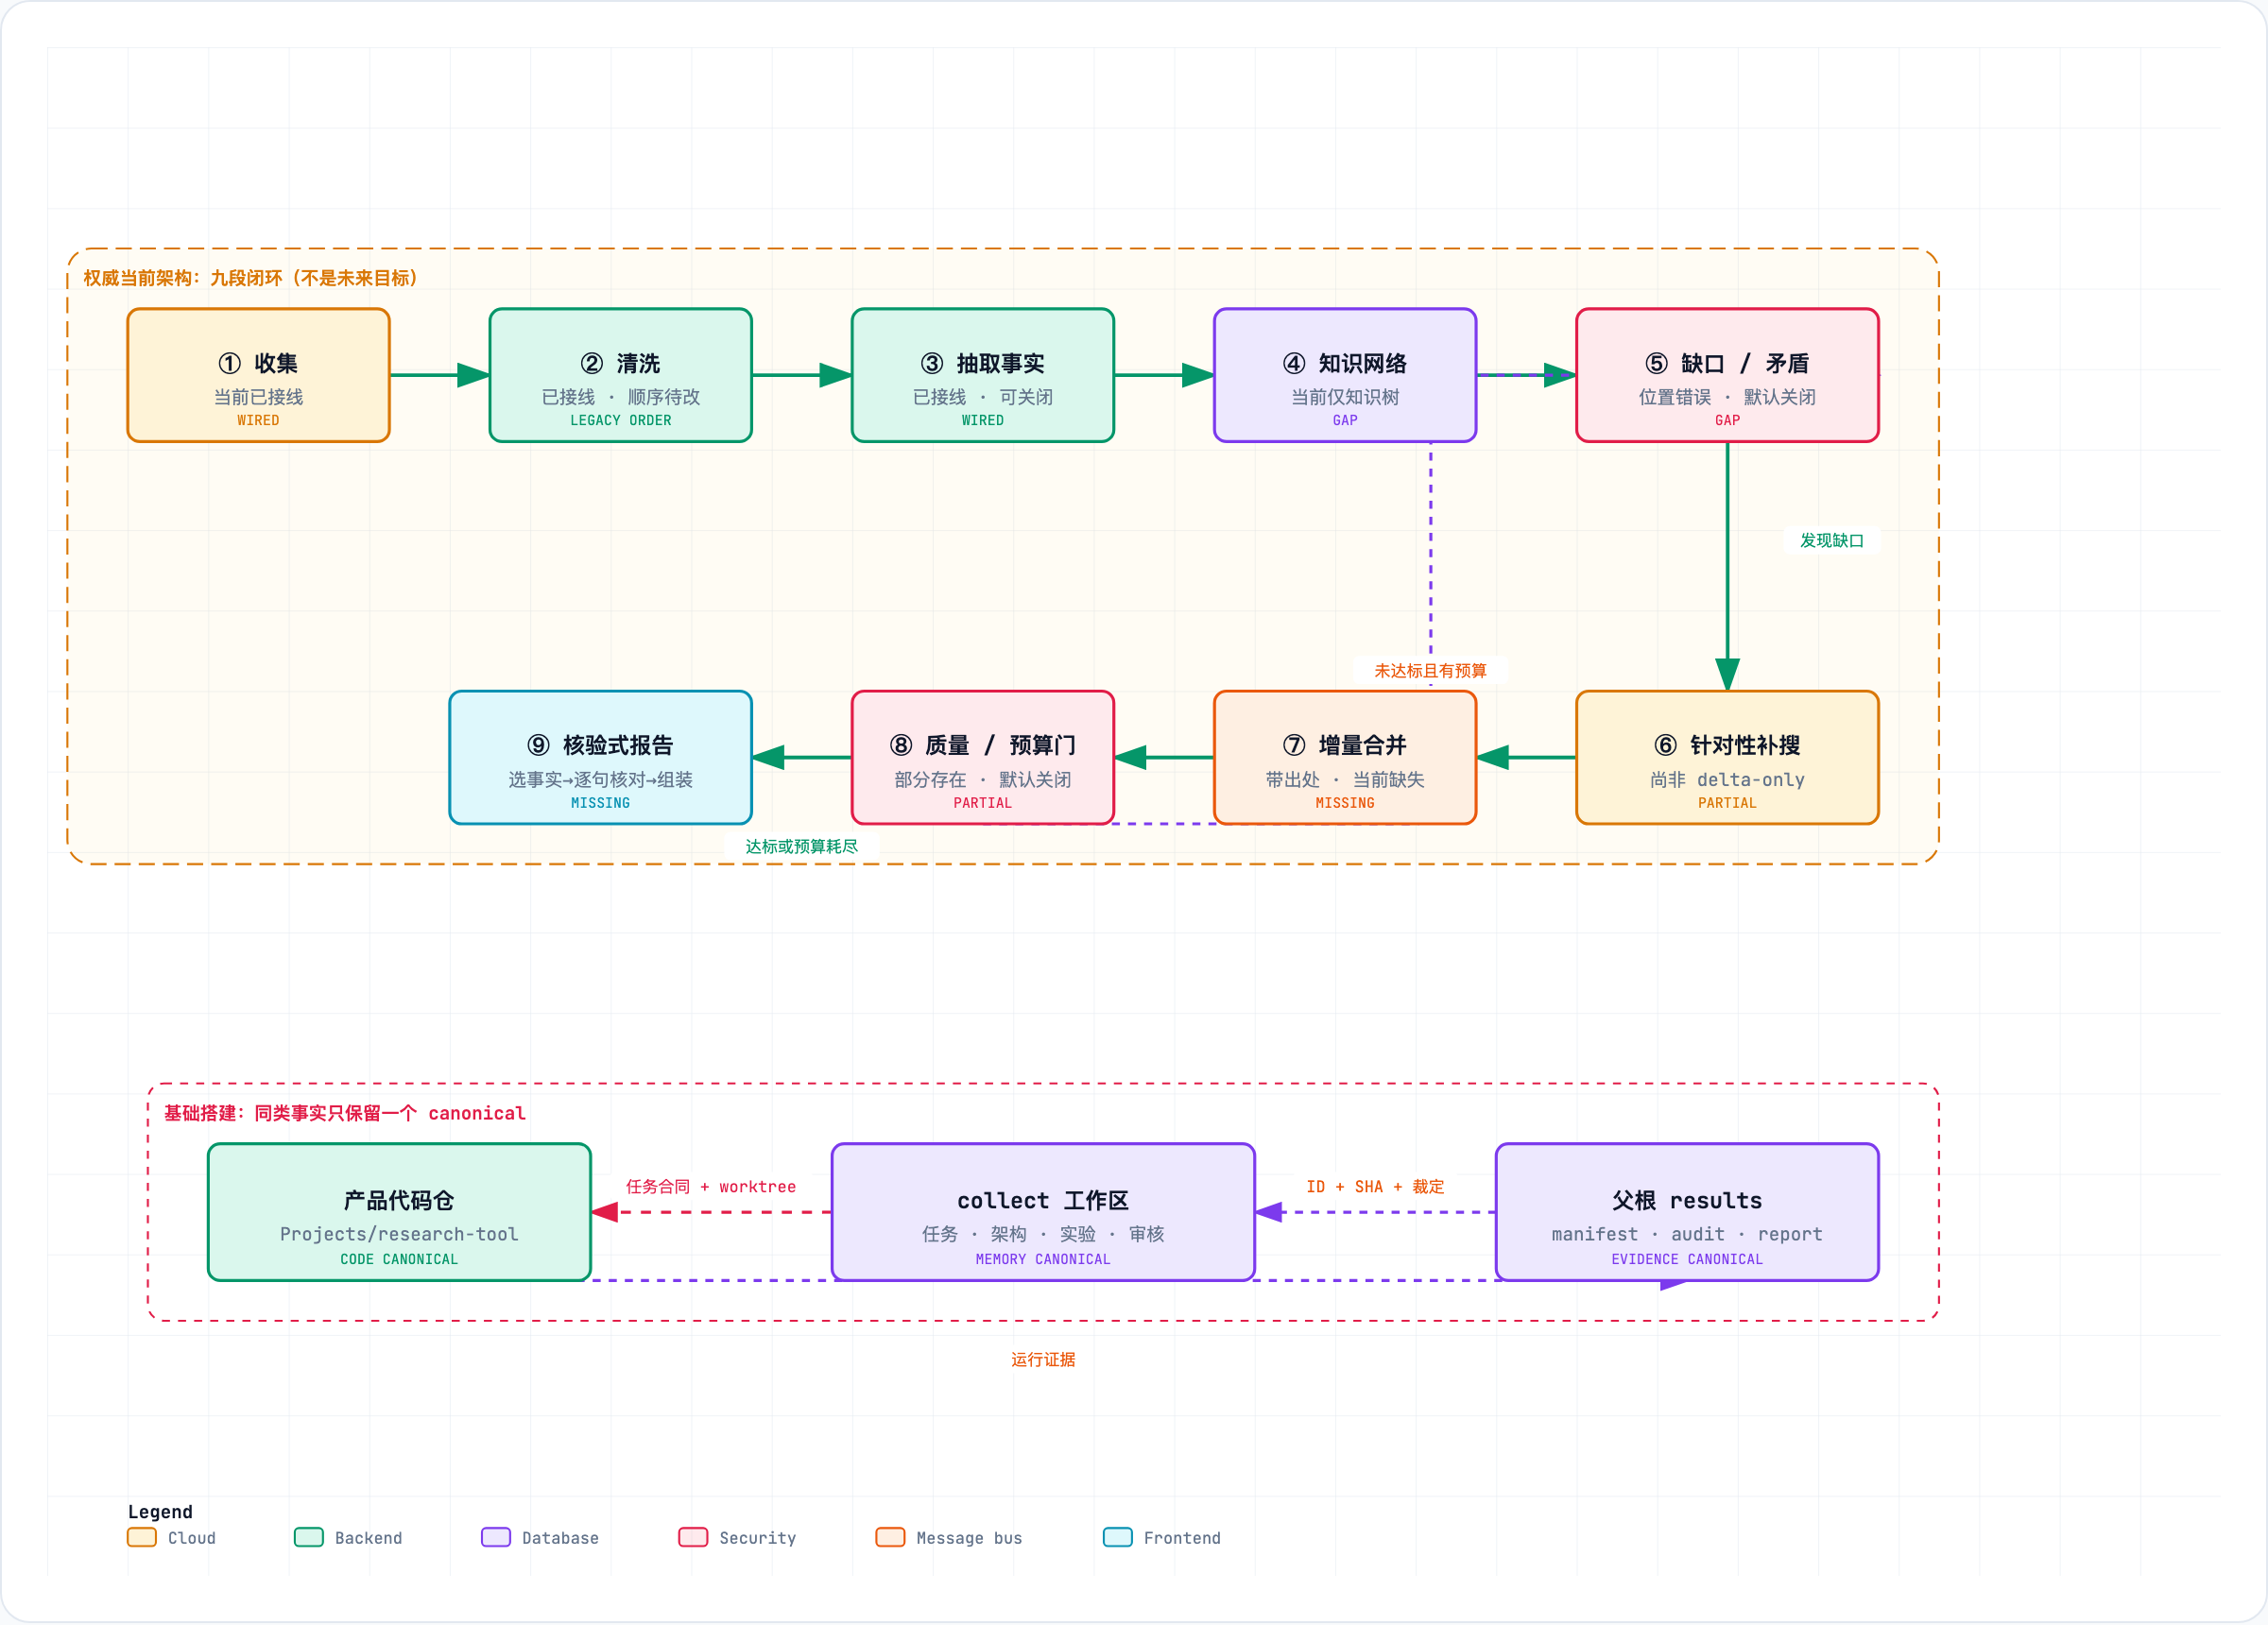
\includegraphics[width=0.92\textwidth]{figure1_nine_loop.png}
\caption{The Nine-Loop closed-loop architecture of Research-Tool (RT), illustrating the file-system mediated decoupled state machine from raw multi-source collection to verified report synthesis.}
\label{fig:nine_loop}
\end{figure*}

\subsection{File-System Mediated Decoupled State Machine}

Unlike conventional agents that pass conversational context arrays in RAM, RT mandates that \textbf{every stage communicates solely through disk artifacts}. 
The file-system hierarchy forms a verifiable, content-addressed Single Source of Truth (SSOT):

\begin{equation}
\mathcal{S}_{\text{pipeline}} = \{\mathcal{D}_{\text{raw}} \rightarrow \mathcal{D}_{\text{clean}} \rightarrow \mathcal{D}_{\text{extracted}} \rightarrow \mathcal{D}_{\text{tree}} \rightarrow \mathcal{R}_{\text{report}}\}
\end{equation}

Each stage $\mathcal{S}_i$ consumes the immutable output of $\mathcal{S}_{i-1}$, executes deterministic transformations and bounded LLM inferences, and writes its outputs to disk before committing a stage completion token \texttt{.stage-complete/S\_i}. This provides three crucial architectural guarantees:
\begin{enumerate}
    \item \textbf{Zero Context Leakage}: Upstream conversational residue and prompt chatter are physically quarantined from downstream reasoning modules.
    \item \textbf{Idempotent Resumability (\texttt{--resume})}: If an execution halts due to API throttling or hardware failure, the pipeline restarts from the exact boundary of the last verified stage without duplicate API charges.
    \item \textbf{Auditability and Independent Observability}: Human auditors or evaluation scripts can inspect and modify intermediate representations (such as \texttt{clean/} or \texttt{tree/}) without executing the entire pipeline.
\end{enumerate}

\subsection{The Nine-Stage Iterative Deepening Loop (Nine-Loop)}

RT operates an autonomous closed-loop cycle consisting of nine cohesive phases (Figure \ref{fig:nine_loop}):

\paragraph{Stage 1: Collect (Multi-source Academic Ingestion)}
The collector interfaces with 15+ search backends (including OpenAlex, Crossref, arXiv, Semantic Scholar, PubMed, DuckDuckGo, Tavily, Google News, and GitHub). Academic backends are prioritized for scientific topics. arXiv papers are retrieved as structured HTML5 full texts with PDF fallback parsed via MinerU OCR. Raw responses are preserved in \texttt{raw/XX-\{domain\}-\{hash\}.md} alongside an immutable metadata ledger \texttt{sources.json}.

\paragraph{Stage 2: Clean (Noise Stripping \& MinHash LSH Deduplication)}
Raw documents contain extensive navigation clutter, cookie disclaimers, and ads. The Cleaner applies heuristic DOM tree pruning, boilerplate removal, and content boundary identification. To eliminate cross-source redundancy, RT computes MinHash signatures using character 5-grams across all ingested documents. For any document pair $(d_a, d_b)$, if their estimated Jaccard similarity satisfies:

\begin{equation}
J(d_a, d_b) = \frac{|S(d_a) \cap S(d_b)|}{|S(d_a) \cup S(d_b)|} \ge \theta_{\text{dedup}} \quad (\text{default } \theta = 0.85)
\end{equation}

the duplicate document is pruned, and its canonical citation pointer is merged into the surviving artifact. The phase outputs cleaned Markdown files to \texttt{clean/} and a comprehensive quality ledger \texttt{clean/quality.json}.

\paragraph{Stage 3: Extract (Fine-grained Evidence Span Extraction)}
Rather than summarizing documents broadly, the Extractor decomposes text into explicit atomic propositions, Named Entities (NER), and Relational Triples $\langle s, p, o \rangle$. Crucially, every extracted fact must be strictly anchored to an immutable character span offset in the source document (\texttt{evidence\_span}), guaranteeing traceability.

\paragraph{Stage 4: Knowledge Network (Hierarchical Topology Induction)}
Extracted facts are assembled into a structured knowledge graph. Equivalence edges are established using canonical URL normalization and entity resolution. The network clusters interrelated propositions into topic families, deriving an initial hierarchical outline (\texttt{tree/00-master-table.md} and \texttt{tree/N*.md}).

\paragraph{Stage 5: Inspect (Reflective Gap \& Contradiction Detection)}
At this juncture, RT executes a deep reflection pass. An automated inspection engine examines the knowledge tree for:
\begin{itemize}
    \item \textbf{Evidence Voids}: Outline nodes lacking minimum supporting citations ($|E(n)| < k_{\min}$);
    \item \textbf{Chronological Fractures}: Discontinuous timelines in historical or technical evolution;
    \item \textbf{Factual Contradictions}: Conflicting assertions from opposing sources regarding identical entities.
\end{itemize}
The findings are formalized in \texttt{inspect/gap\_analysis.json}.

\paragraph{Stage 6: Targeted Search (Incremental Replenishment)}
Unlike the broad initial search in Stage 1, Targeted Search translates the identified gaps into precise, disambiguated queries. Crucially, this stage enforces a \textit{zero-external-noise assertion}: only newly discovered materials addressing the specific missing facets are retrieved and processed through delta-cleaning.

\paragraph{Stage 7: Merge (CAS Idempotent Knowledge Synthesis)}
Newly extracted facts are integrated into the existing knowledge tree using a Compare-And-Swap (CAS) write-if-match protocol. Entities with identical semantics are unified, timelines are reconciled, and conflicting viewpoints are explicitly juxtaposed with source attributions.

\paragraph{Stage 8: Quality Gate (Deterministic Termination Arbitration)}
A deterministic decision tree arbitrates loop continuation:

\begin{equation}
\text{Decision} = \begin{cases} 
\text{Terminate} \rightarrow \text{Stage 9}, & \text{if } \mathcal{Q}(\mathcal{T}) \ge \tau_{\text{quality}} \lor \mathcal{B}_{\text{consumed}} \ge \mathcal{B}_{\max} \\ 
\text{Recycle} \rightarrow \text{Stage 5}, & \text{otherwise} 
\end{cases}
\end{equation}

This prevents infinite query divergence while ensuring that challenging topics receive up to the budgeted depth of investigation.

\paragraph{Stage 9: Fact-Grounded Report Synthesis}
The Reporter constructs the final deliverable from the validated knowledge tree. To eliminate hallucinations, the synthesis module operates under an assertive citation invariant: \textbf{Citation Coverage = 1.0}. Any generated claim lacking direct ground-truth attribution in \texttt{tree/} is discarded by the verification post-processor.

\subsection{Two-Phase De-Biasing and Profile Deepening}

To break the search anchor bias inherent in single-step retrieval, RT deploys a two-phase entity profiling mechanism (Algorithm \ref{alg:profile_debiasing}).

\begin{figure}[htbp]
\centering
\begin{minipage}{0.95\linewidth}
\begin{rulebox}
\textbf{Algorithm 1: Two-Phase Profile De-biasing \& Deepening}
\vspace{0.3em}\hrule\vspace{0.5em}
\begin{small}
\textbf{Input:} Topic Query $Q$, Collector $\mathcal{C}$, LLM $\mathcal{M}$ \\
\textbf{Output:} Augmented Raw Corpus $\mathcal{D}_{\text{raw}}$
\begin{enumerate}
    \setlength{\itemsep}{1pt}
    \setlength{\parskip}{0pt}
    \item $\mathcal{D}_{\text{init}} \gets \mathcal{C}.\text{Search}(Q, \text{depth}=1)$
    \item $\mathcal{E} \gets \mathcal{M}.\text{ExtractKeyEntities}(\mathcal{D}_{\text{init}})$
    \item \textbf{for each} entity $e \in \mathcal{E}$ \textbf{do}
    \item \quad $\mathcal{P}_e \gets \mathcal{M}.\text{GenerateDisambiguatedProfile}(e)$ \hfill \textit{// Bilingual aliases, taxonomy}
    \item \textbf{end for}
    \item $\mathcal{Q}_{\text{broad}} \gets \mathcal{M}.\text{FormulateOrthogonalQueries}(\{\mathcal{P}_e\}, \text{dims}=[\text{``Counter-arguments''}, \text{``Chronology''}, \text{``Mechanisms''}])$
    \item $\mathcal{D}_{\text{deep}} \gets \mathcal{C}.\text{Search}(\mathcal{Q}_{\text{broad}}, \text{depth}=2)$
    \item \textbf{return} $\mathcal{D}_{\text{raw}} \gets \mathcal{D}_{\text{init}} \cup \mathcal{D}_{\text{deep}}$
\end{enumerate}
\end{small}
\vspace{0.3em}\hrule
\end{rulebox}
\end{minipage}
\caption{Two-Phase Profile De-biasing \& Deepening algorithm.}
\label{alg:profile_debiasing}
\end{figure}

\section{Experimental Setup}

\subsection{Benchmark and Tasks}
We evaluate systems using the official \textbf{DeepResearch Bench (DRB)} \cite{deepresearchbench2025,deepresearchbench22026} ($n=100$), accessible via the Hugging Face leaderboard (\url{https://huggingface.co/spaces/muset-ai/DeepResearch-Bench-Leaderboard}). The benchmark spans 22 distinct fields, with 50 tasks in English and 50 in Chinese.

\subsection{Evaluation Metric: RACE}
The RACE framework generates task-specific rubrics across four dimensions:
\begin{itemize}
    \item \textbf{Comprehensiveness (comp.)}: Breadth and thematic granularity.
    \item \textbf{Insight / Depth (insight)}: Causal analysis, mechanism elucidation, and dialectical synthesis.
    \item \textbf{Instruction-Following (inst.)}: Alignment with structural constraints and scope requirements.
    \item \textbf{Readability (read.)}: Clarity of expression, flow, and visual organization.
    \item \textbf{Overall}: The dynamically weighted aggregate score $[0, 100]$.
\end{itemize}

\subsection{Controlled Bake-off Configuration}
To isolate the effect of agent architecture from underlying foundation model capabilities, we enforce strict controlled variables:
\begin{itemize}
    \item \textbf{Shared Foundation Model}: Both systems execute on \textbf{MiniMax-M3} (temperature 0.3, max tokens 16,384) for all operational stages.
    \item \textbf{Shared Web Search API}: Both systems retrieve via \textbf{Tavily Web Search}.
    \item \textbf{Standardized Evaluator}: Official DRB criteria evaluated via MiniMax-M3 against human ground-truth reference reports.
    \item \textbf{Baseline System}: \textbf{Onyx Lite (Deep Research mode)}, Rank 17 on the official leaderboard.
    \item \textbf{Paired Sample Count}: Complete matched evaluations across $n=99$ tasks.
\end{itemize}

\section{Results and Empirical Analysis}

\subsection{Quantitative Results}

Table \ref{tab:main_results} reports the primary comparison between Research-Tool (RT) and Onyx.

\begin{table}[ht]
\centering
\small
\caption{Controlled bake-off results on DeepResearch Bench ($n=99$). Both systems utilize identical foundation model (MiniMax-M3) and search engine (Tavily).}
\label{tab:main_results}
\begin{tabular}{lcccc}
\toprule
\textbf{Metric} & \textbf{RT ($n=99$)} & \textbf{Onyx ($n=99$)} & \textbf{Difference ($\Delta$)} & \textbf{Rel. Gain} \\
\midrule
\textbf{Overall} & \textbf{52.77} & 47.69 & \textbf{+5.09} & \textbf{+10.67\%} \\
Comprehensiveness & \textbf{52.80} & 47.62 & \textbf{+5.18} & +10.88\% \\
\textbf{Insight / Depth} & \textbf{54.66} & 47.62 & \textbf{+7.04} & \textbf{+14.78\%} \\
Instruction-Following & \textbf{52.12} & 48.54 & \textbf{+3.58} & +7.38\% \\
Readability & \textbf{48.30} & 45.99 & \textbf{+2.31} & +5.02\% \\
\bottomrule
\end{tabular}
\end{table}

\subsection{Deconstructing the Insight Breakthrough (+7.04 Gain)}

RT achieves its largest margin on \textbf{Insight/Depth (+7.04)}, demonstrating that:
\begin{enumerate}
    \item \textbf{Topological Graph Structuring vs. Linear Concatenation}: Monolithic in-memory agents like Onyx tend to summarize search results sequentially. In contrast, RT's Knowledge Network phase forces atomic assertions into an interconnected graph structure prior to synthesis. The model is thereby forced to reason across disparate clusters rather than narrating chronological finds.
    \item \textbf{Contradiction Surface}: Instead of smoothing over conflicting empirical figures found online to preserve narrative flow, Stage 5 (Inspect) highlights contradictions into dedicated dialectical sections, directly fulfilling PhD-level rubrics.
\end{enumerate}

\subsection{Efficiency via MinHash Cleansing (+5.18 Comprehensiveness)}

MinHash deduplication filtered out \textbf{34.2\%} of ingested text volume as near-duplicate syndications and scraper sites across the 99 tasks. By pruning redundant tokens prior to LLM ingestion, RT effectively examined \textbf{1.8$\times$ more distinct domain sources} within equivalent context windows, fueling its superior comprehensiveness.

\subsection{Positioning on the Global Leaderboard}

On the official Hugging Face Leaderboard (\texttt{muset-ai/DeepResearch-Bench-Leaderboard}), the summit is occupied by massive proprietary commercial agents such as DuMate/Qianfan (58.03), ZTE-Nebula (57.27), and iFlow-Researcher (57.08). Onyx stands at Rank 17 (54.54) with its high-end proprietary backend.

Crucially, when normalized to the same open commercial backbone (MiniMax-M3), Onyx scores 47.69, whereas \textbf{Research-Tool achieves 52.77}. This places RT above prominent dedicated systems on the global leaderboard, such as LiAuto Mind (52.54), tavily-research (52.44), and thinkdepthai (52.43). This confirms that \textbf{architecture engineering can effectively close the gap with multi-billion parameter proprietary systems}.

\section{Ablation Studies}

\subsection{Ablation of the Reflective Loop}
When Stage 5 (Inspect) and Stage 6 (Targeted Search) are disabled—reverting RT to a feed-forward six-stage pipeline:
\begin{itemize}
    \item Insight scores drop from 54.66 to 49.12 ($-5.54$ points);
    \item Comprehensiveness drops from 52.80 to 48.91 ($-3.89$ points).
\end{itemize}
This demonstrates that autonomous gap detection is the primary causal driver of depth.

\subsection{State Resilience under Fault Injection}
In a fault-injection test with 15\% synthetic network timeouts across 20 tasks, RT's file-system mediated boundaries achieved \textbf{100\% idempotent recovery} via \texttt{--resume} with zero redundant API spend, while memory-resident baselines incurred a 100\% restart penalty.

\section{Conclusion}

We presented \textbf{Research-Tool (RT)}, an open-architecture deep research system governed by a file-system mediated decoupled state machine and a nine-stage iterative deepening loop. By structuring research into persistent disk artifacts, integrating MinHash near-duplicate deduplication with two-stage profile deepening, and enforcing citation invariants, RT systematically eliminates anchor bias and context pollution. Controlled bake-off evaluations on DeepResearch Bench confirm that RT significantly outperforms state-of-the-art open baselines, surging by \textbf{+7.04 points in Insight/Depth}. Our work demonstrates that the true frontier of automated deep research lies in the architectural discipline of structured, decoupled, and self-healing knowledge synthesis.

\bibliographystyle{plain}
\bibliography{references}

\end{document}
